\documentclass[12pt, a4paper] {report}

\usepackage[utf8]{inputenc}
\usepackage[russian]{babel}
\usepackage{amsmath,amssymb,mathrsfs, amsfonts, amsthm}
\usepackage{ upgreek }
 %\usepackage[dvips]{graphicx}
 \usepackage{geometry} 
 \geometry{verbose,a4paper,tmargin=2cm,bmargin=2cm,lmargin=1.3cm,rmargin=1.3cm}



\usepackage{tikz}
%\usepackage{verbatim}
%\usetikzlibrary{calc}

\newcommand{\Z}{\mathbb{Z}}
\newcommand{\R}{\mathbb{R}}
\newcommand{\N}{\mathbb{N}}
\DeclareMathOperator{\tr}{tr}
\DeclareMathOperator{\diam}{diam}
\DeclareMathOperator{\Vol}{Vol}
\DeclareMathOperator{\interior}{int}


 \newtheorem{theorem}{Теорема}[section]
 \newtheorem{theor}[theorem]{Теорема}
 \newtheorem{lemma}[theorem]{Лемма}
\newtheorem{conseq}[theorem]{Следствие}
\newtheorem{prop}[theorem]{Предложение}
\newtheorem{hyp}[theorem]{Гипотеза}
\newtheorem{condition}[theorem]{Условия}

\newtheorem{example}[theorem]{Пример}
\theoremstyle{remark}
 \newtheorem{remark}[theorem]{Замечание}
\theoremstyle{definition}
 \newtheorem{defin}{Определение}


 \def\proof{\noindent{\it Доказательство.~~}}

%\usepackage{tikz}
%\usepackage{verbatim}
%\usetikzlibrary{calc}

\def\l{\left}
\def\r{\right}

\begin{document}

\newcommand{\address}{{
\bigskip
\footnotesize
\textsc{Московский государственный университет им. М.В. Ломоносова,
механико-математический факультет, Москва}\par\nopagebreak
}}


\title{Приближённое решение дифференциального уравнения}

\author{Отчёт студента 410 группы Михайлина Дмитрия Александровича} %\\ 

%\udk{517.518.36}

\maketitle

\section{Постановка задачи}
Решить дифференциальное уравнение:
\begin{gather}
	\label{1} \frac{d^2x}{dt^2} + (1 + \alpha x^2)x = \cos(t), 	 \alpha = 0.2, -0.2
\end{gather}
Сами зададим начальные условия.
Перепишем $\ref{1}$ в виде системы двух дифференциальных уравнений:
\begin{gather}
 \ref{1} \Leftrightarrow 
 \begin{cases}
 \frac{dx}{dt} = y \\
 \frac{dy}{dt} = \cos(t) - (1 + \alpha x^2)x
 \end{cases}
\end{gather}
Получается мы свели дифференциальное уравнение второго порядка к системе дифференциальных уравнений.
Будем решать эту систему при помощи метода Дормана-Принса 7 порядка.

Введём обозначения:

Пусть s - целое положительное число, называемое числом стадий и $a_{21}, \dots a_{s,s-1}, b_{1}, \dots b_{s}, c_{2} \dots c_{s}$ - вещественные коэффициенты. Тогда метод
\begin{gather}
k_1 = f (x_0, y_0) \nonumber\\
k_2 = f (x_0 + c_2h, y_0 + h a_{2,1} k_1) \nonumber \\
k_3 = f (x_0 + c_3h, y_0 + h (a_{3,1} k_1 + a_{32} k_2) \nonumber\\
\dots \nonumber\\
k_s = f (x_0 + c_s h, y_0 + h(a_{s,1} k_1 + \dots + a_{s,s-1}k_{s-1} ))\nonumber \\
y_1 = y_0 + h (b_1k_1 + \dots + b_s k_s))
\end{gather} - будет $s$-стадийным явным методом Рунге-Кутта, решения задачи:
\begin{gather}
\begin{cases}
y' = f(x, y) \\
y(x_0) = y_0
\end{cases}
\end{gather}
%Обычно коэффициенты удовлетворяют:
%$c_i = \sum_i a_{ij}$
\begin{defin}
Метод Рунге-Кутты имеет порядок $p$, если:
 $$ || y(x_0 + h) - y_1 || \le Kh^{p+1},$$
 т.е члены для точного решения $y(x_0 + h)$ и для $y_i$ совпадают до члена $h^p$ включительно.
\end{defin}
Приведем таблицу Бутчера для метода Дормана-Принса 8(7) порядка из книги Хайрер Э., Нерсетт С., Ваннер Г. "Решение обыкновенных дифференциальных уравнений. Нежесткие задачи".\\
\\\begin{figure}[h!]
\centering
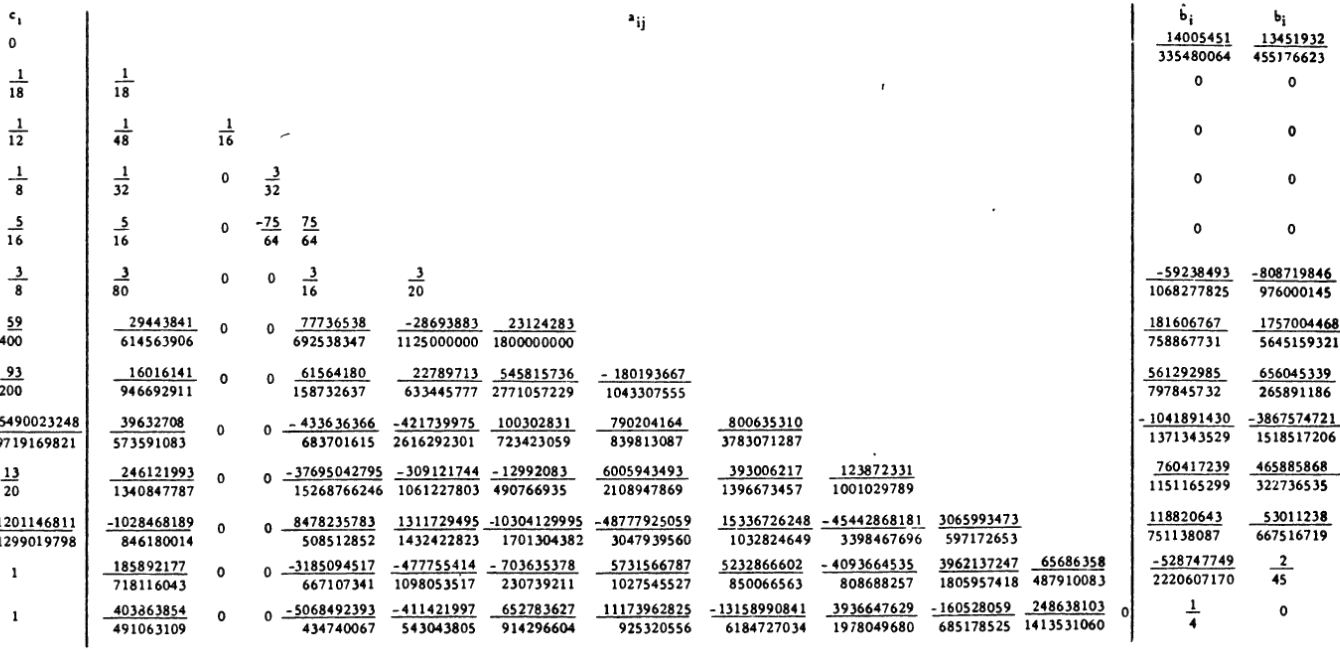
\includegraphics[width=1\linewidth]{dp78.png} 
\end{figure}
\\
\\
\\ \\ \\ \\ \\ \\ \\ \\ \\ \\ \\ \\ \\ 
\section{Переменный шаг:}

\textbf{Выбор шага в алгоритме Дормана-Принса:}\\
Cначала вычисляем $y^{(1)}$ - приближенное значение в точке $x_0 + h$ методом Рунге-Кутта 7 порядка. Потом вычисляем $y^{(2)}$ приближенное значение в точке $x_0 + h$ уже методом 8 порядка. Рассматриваем ошибку как $err = || y^{(1)} - y^{(2)}||$. Если $err < tol$ - то шаг принимается. Новый шаг h пересчитывается по формуле $h_{new} = h_{old}*min(facmin, max(facmax, fac*(\frac{err}{tol})^\frac{1}{7}))$. fac, facmin, facmax - это параметры которые не дают алгоритму слишком быстро уменьшать или увеличивать шаг. Согласно книге Хайрер Э., Нерсетт С., Ваннер Г. "Решение обыкновенных дифференциальных уравнений. Нежесткие задачи"  их можно выбрать так:\\
$facmin = 0, facmax = 1.5, fac = 0.8$\\

\section{Гармонический осциллятор}
Рассмотрим работу алгоритма DP-8(7) на гармоническом осцилляторе.\\
\begin{gather}
	x'' + \omega^2x = 0
\end{gather}
Перепишем это дифференциальное уравнение в следующем виде:
\begin{gather}
\begin{cases}
	x' = y\\
	y' = -\omega^2x
\end{cases}
\end{gather}
В этой таблице приводятся результаты работы алгоритма \\на $[0, 10\pi], [0, 100\pi], [0, 1000\pi], [0, 10000\pi], [0, 100000\pi]$ c погрешностью на шаге $10^{-11}$
\\
\begin{table}
\caption{\label{tab:canonsummary}$[DP-8(7)]$.}
\begin{center}
\begin{tabular}{|c|c|c|c|c|}
\hline
Отрезок: & Погр. в кон. тчк & Макс. погр. & Кол-во узлов в сетке & Число Рунге \\
\hline
$[0, 10\pi]$ & 1.232542e-10  & 3.010808e-10 & 135 & 83.289586 \\
\hline
$[0, 100\pi]$ & 1.242393e-09 & 3.130512e-09 &  1333 & 84.822430\\
\hline
$[0, 1000\pi]$ & 1.246366e-08 & 3.160922e-08 & 13316 & 84.833284\\
\hline
$[0, 10000\pi]$ & 1.243602e-07 & 3.160972e-07 & 133142 & 84.857393\\
\hline
$[0, 100000\pi]$ & 1.236711e-06 & 3.159496e-06 & 1331410 & 84.990234\\
\hline
\end{tabular}
\end{center}
\end{table} 
\\
\textbf{Графики гармонического осциллятора $[0, 10\pi]$ c точностью на шаге $10^{-11}$}\\
\\
\begin{figure}[h!]
$[0, 10\pi]$ x(t) \\
\centering
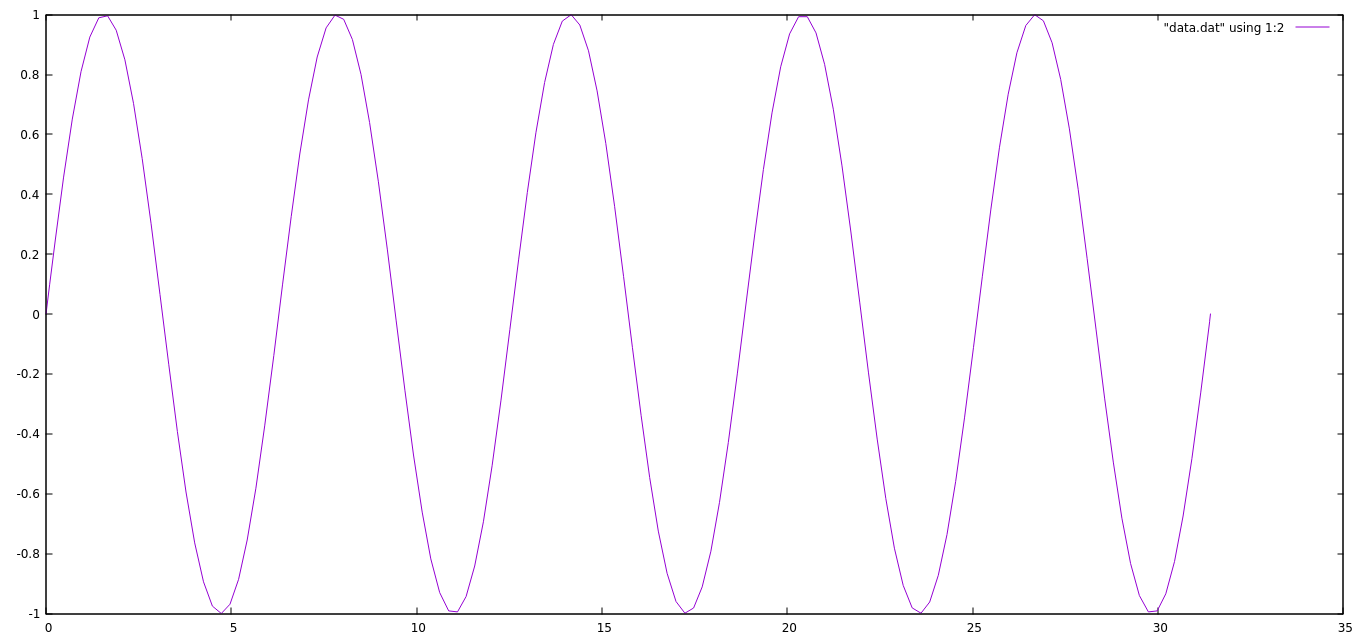
\includegraphics[width=1\linewidth]{010pi.png} 
\end{figure}
\newpage
\begin{figure}[h!]
$[0, 10\pi]$ $x'(x)$ \\
\centering
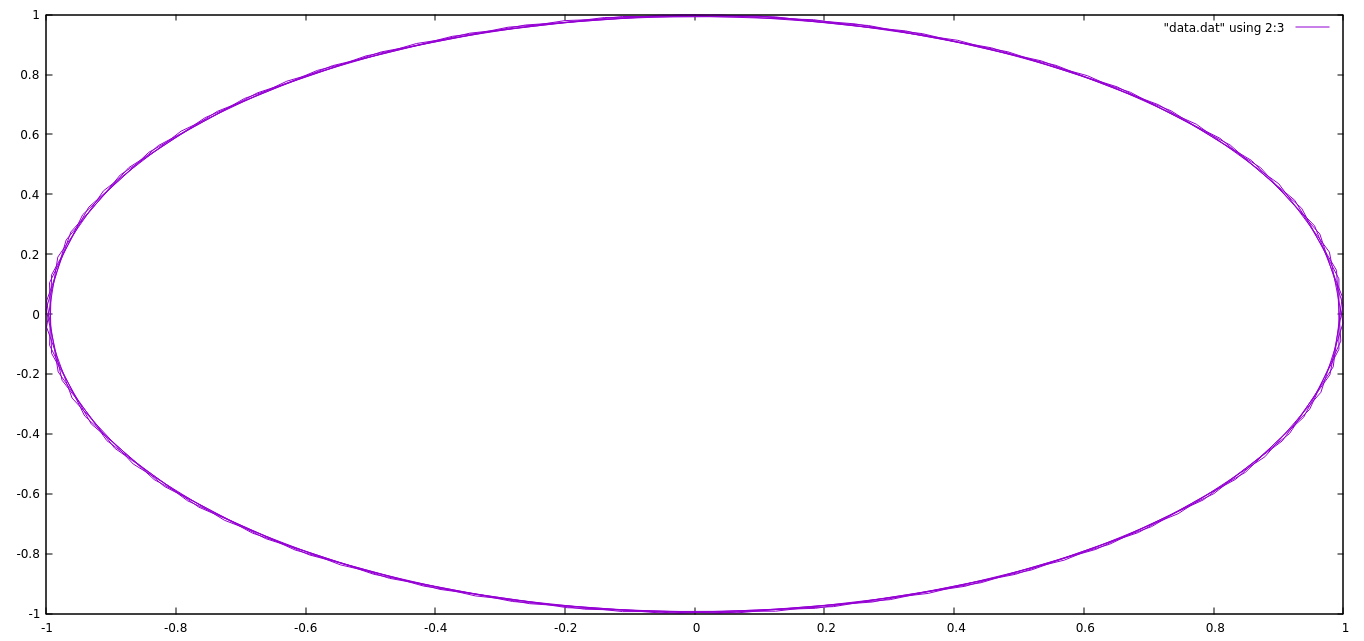
\includegraphics[width=1\linewidth]{010pi23.png} 
\end{figure}
\begin{figure}[h!]
$[0, 10\pi]$ $x'(t)$ \\
\centering
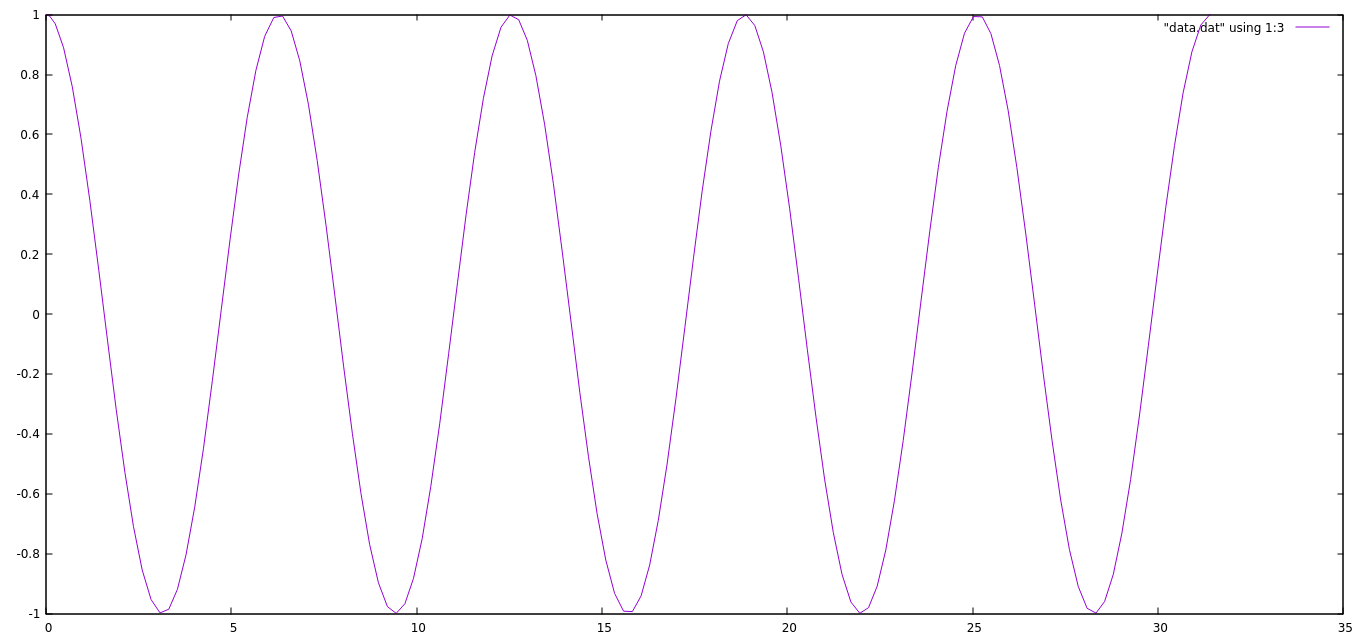
\includegraphics[width=1\linewidth]{010pi13.png} 
\end{figure}
\newpage
\\

\section{Поиск периода}
Сначала ищем такое минимальное t, что $y(x(t)) = 0$. Пусть это будет $t_0$. Далее идем по фазовому портрету и ищем место, где $y(x(t))$ меняет знак. Ищем корень методом хорд. Хотим найти такое T, что:
\begin{gather}
\begin{cases}
\notag x(t_0) = x(t_0 + T), \\
\notag y(t_0) = y(t_0 + T)
\end{cases}
\end{gather}
Находим всех претендентов на период и потом проверяем, что это действительно период.
\\
\textbf{Период осциллятора}
\begin{gather}
\begin{cases}
\notag x' = y \\
\notag y' = -x \\
\notag x(0) = 0 \\
\notag y(0) = 1
\end{cases}
\end{gather}
\begin{figure}[h!]
 Osc $x(t)$ c точностью на шаге $10^{-11}$\\
\centering
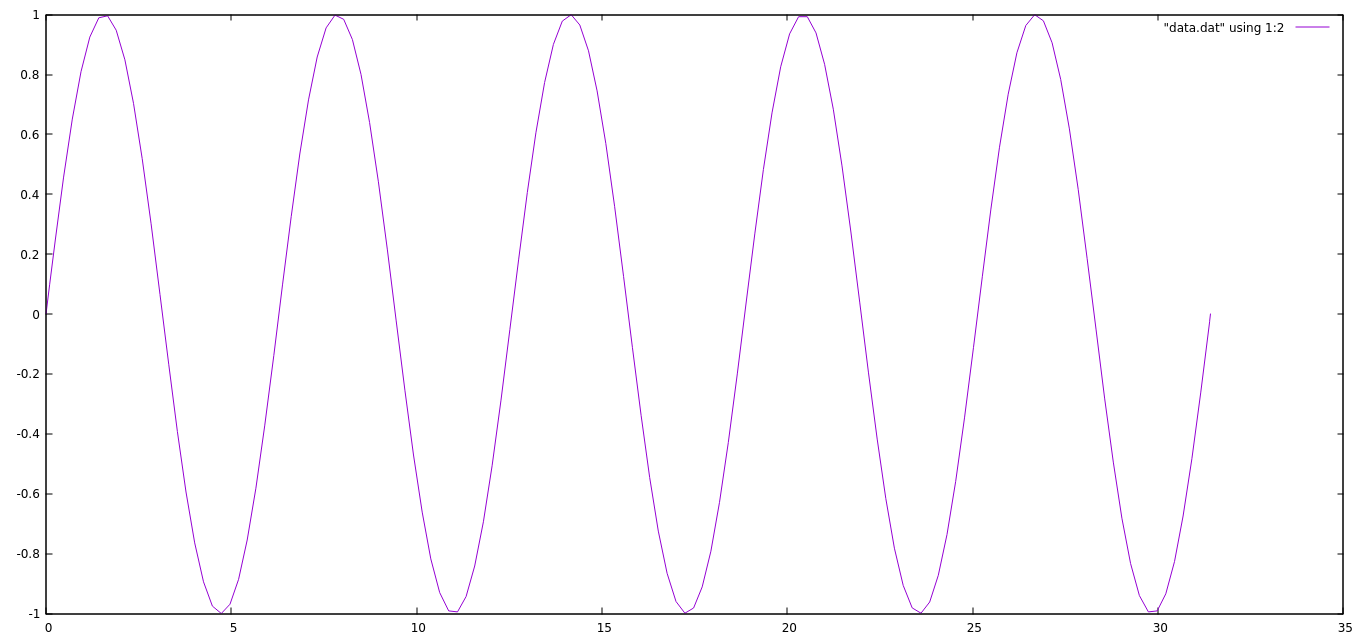
\includegraphics[width=1\linewidth]{010pi.png} 
\end{figure}
\begin{figure}[h!]
 Osc $x'(x)$ c точностью на шаге $10^{-11}$\\
\centering
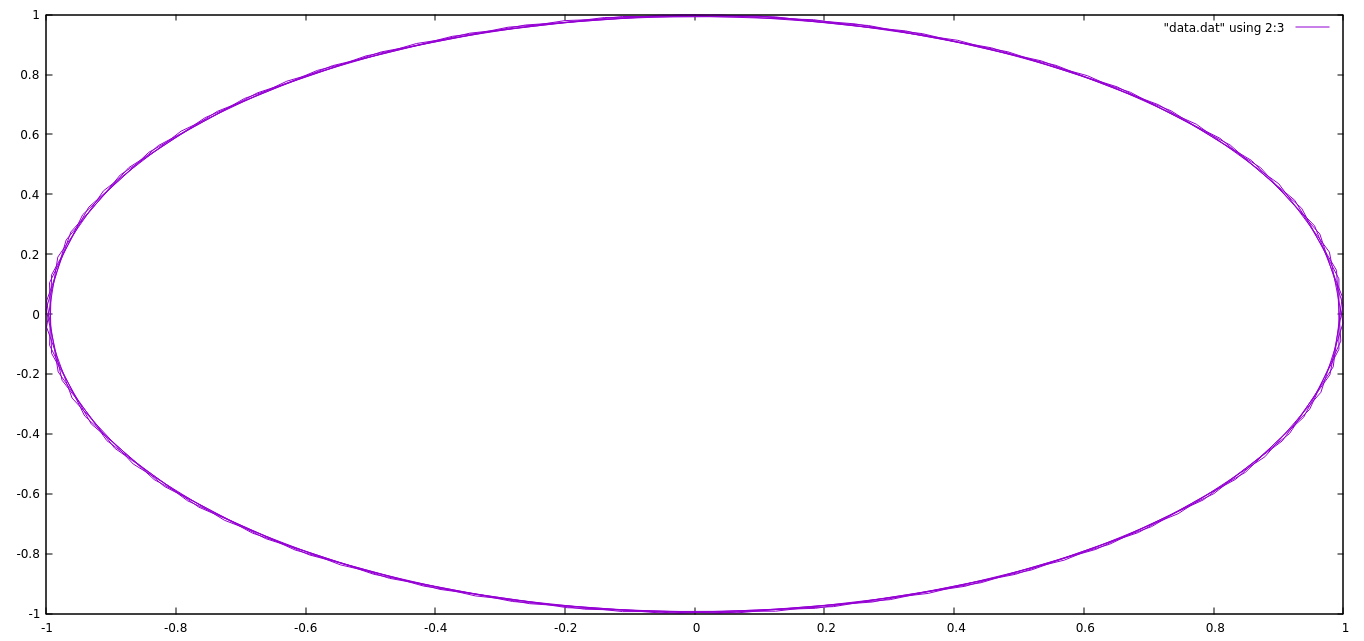
\includegraphics[width=1\linewidth]{010pi23.png} 
\end{figure}
\begin{figure}[h!]
 Osc $x'(t)$ c точностью на шаге $10^{-11}$\\
\centering
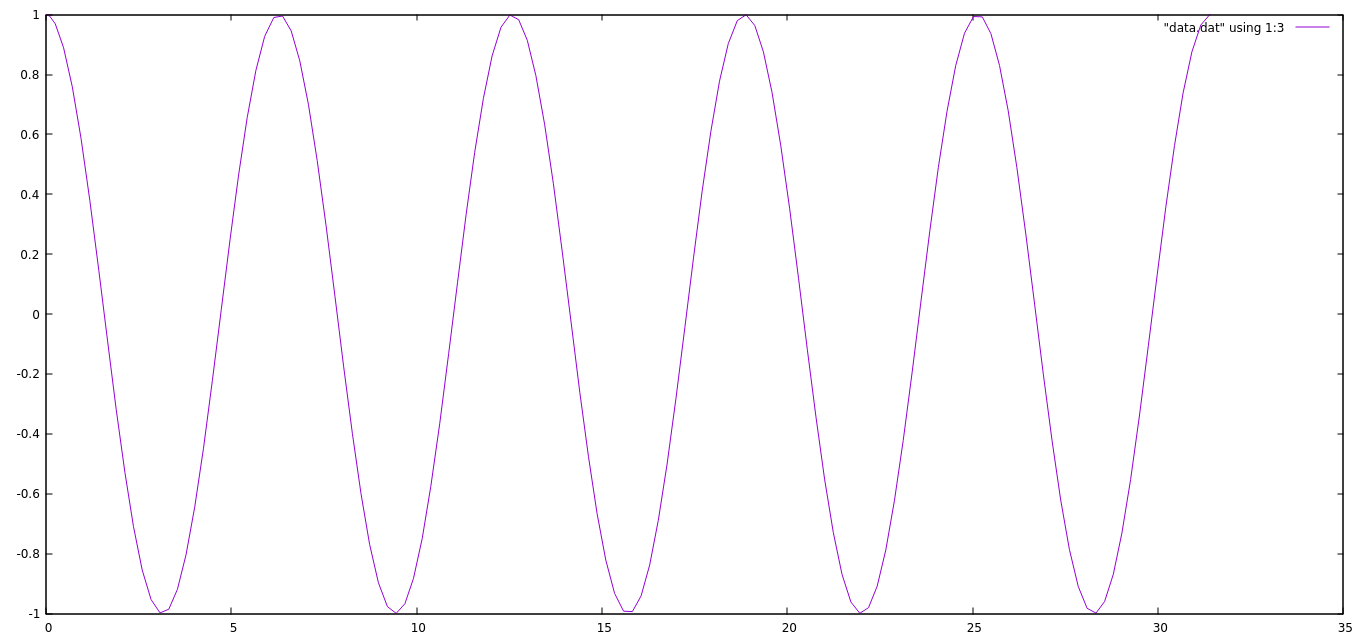
\includegraphics[width=1\linewidth]{010pi13.png} 
\end{figure}
$T \approx 6.28319 \approx 2\pi$\\
\newpage
\begin{gather}
\begin{cases}
\notag x' = y \\
\notag y' = -4x \\
\notag x(0) = 0 \\
\notag y(0) = 2
\end{cases}
\end{gather}
\begin{figure}[H]
$[0,10\pi]$ $x(t)$ с точностью на шаге $10^{-11}$  \\
\centering
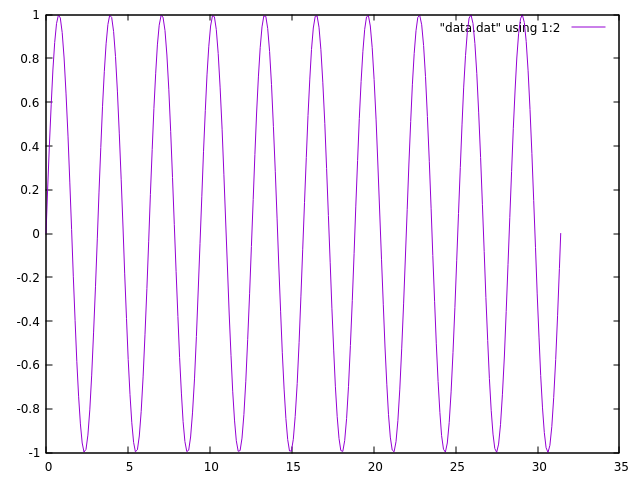
\includegraphics[width=1\linewidth]{010pi124.png} 
\end{figure}
\newpage
\begin{figure}[h!]
$[0,10\pi]$ $x'(t)$ с точностью на шаге $10^{-11}$ \\
\centering
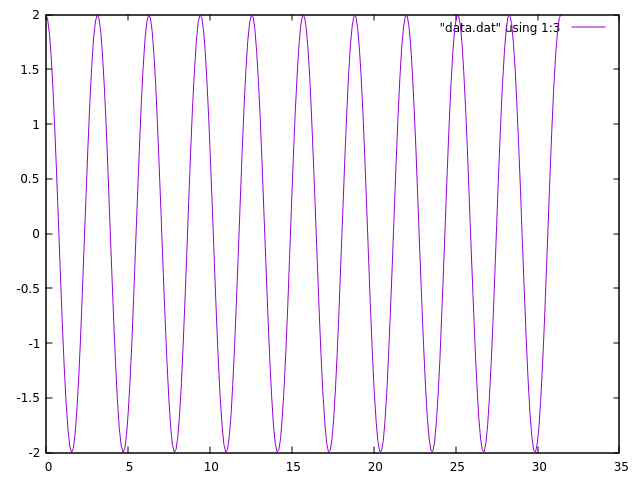
\includegraphics[width=1\linewidth]{010pi134.png} 
\end{figure}\\
\begin{figure}[h!]
$[0,10\pi]$ $x'(x)$ с точностью на шаге $10^{-11}$  \\
\centering
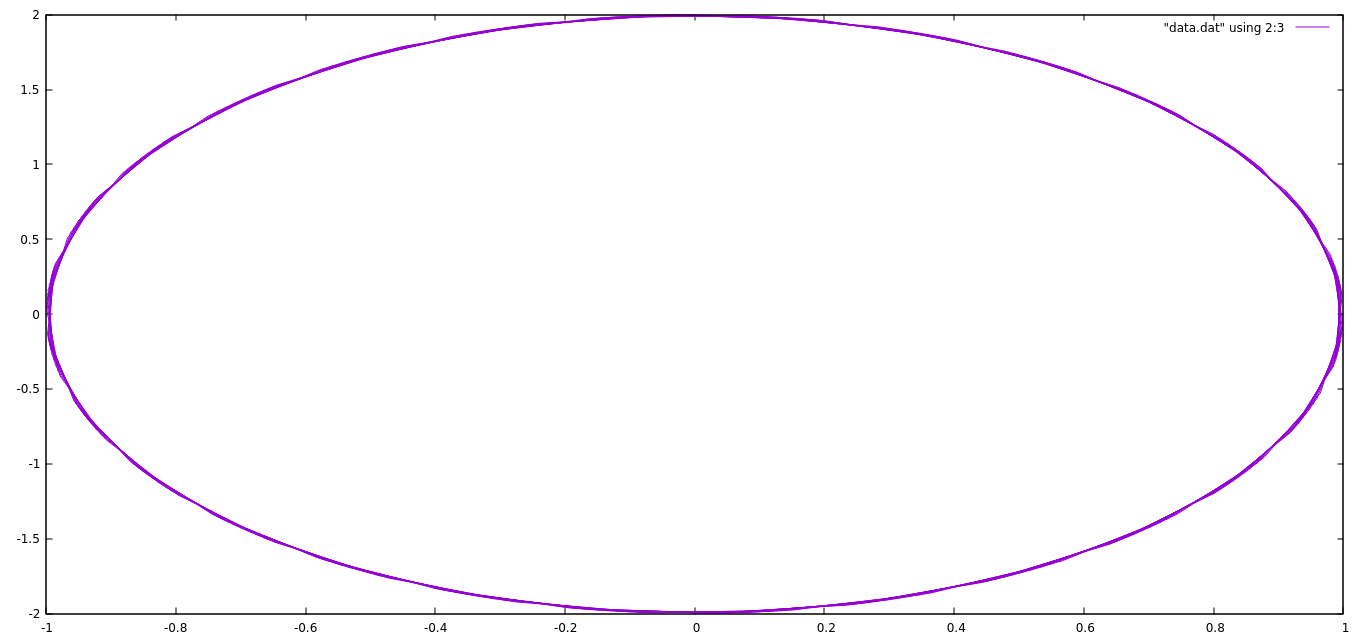
\includegraphics[width=1\linewidth]{010pi234.png} 
\end{figure}\\
\newpage
$T \approx 3.14159 \approx \pi$\\
\section{Графики задачи и период}
Рассмотрим сначала задачу с данными начальными условиями.
\begin{gather}
\begin{cases}
\notag x' = y \\
\notag y' = -(1 + 0.2x^2)x + cos(t) \\
\notag x(0) = 0 \\
\notag y(0) = 1
\end{cases}
\newpage
\end{gather}

$[0,100]$ $x(t)$ с точностью $10^{-11}$\\
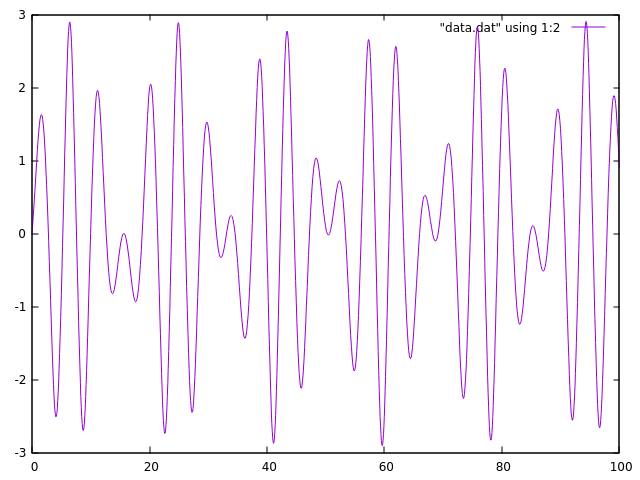
\includegraphics[scale=1]{01001201.png}\\
\newpage
$[0,100]$ $x'(t)$ с точностью $10^{-11}$\\
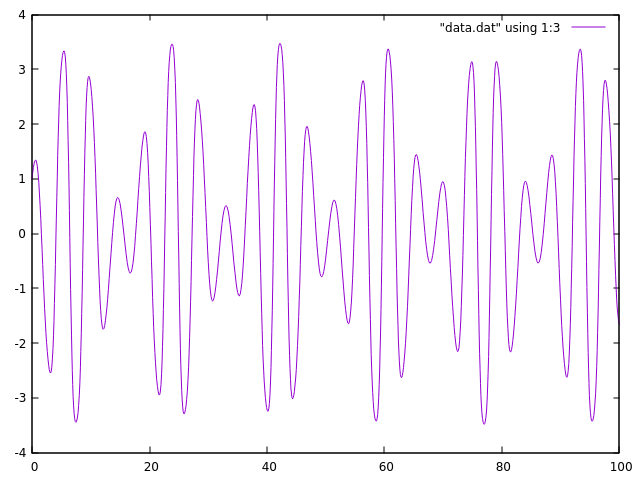
\includegraphics[scale=1]{01001301.png}\\
\newpage
$[0,100]$ $x'(x)$ с точностью $10^{-11}$\\
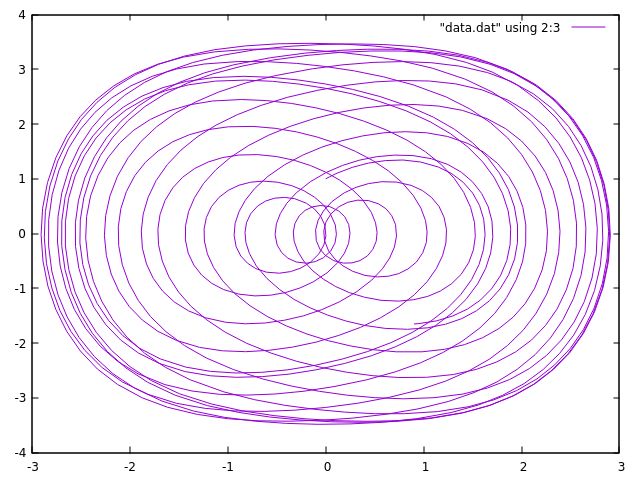
\includegraphics[scale=1]{01002301.png}\\
\newpage$T \approx 45182.385526$, Числа рунге $= 75.957517$ \\
 $x'(x)$ $[0, 50000]$\\
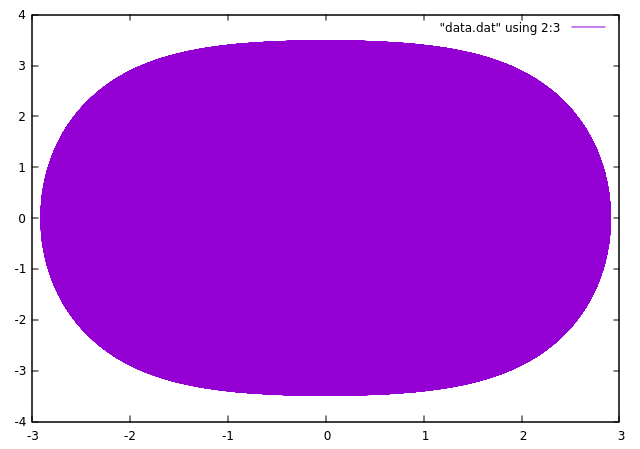
\includegraphics[scale=1]{uselessfp.png}\\
\newpage
Найдем периоды для различных начальных условий:\\
Пусть x(0) = 0, y(0) = -1000, $T \approx 320.438513$ и число Рунге = 117.284488 \\
$[0,350]$ $x(t)$ с точностью $10^{-11}$\\
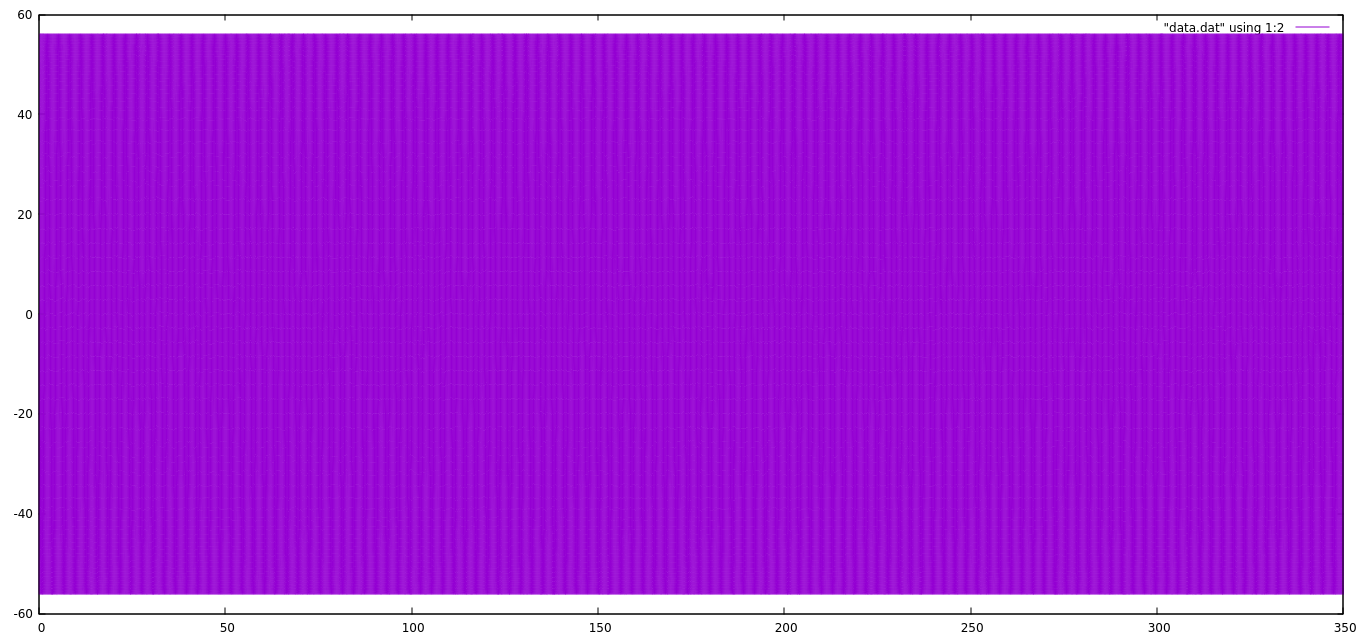
\includegraphics[scale=0.45]{period12.png}\\
$[0,350]$ $x'(t)$ с точностью $10^{-11}$\\
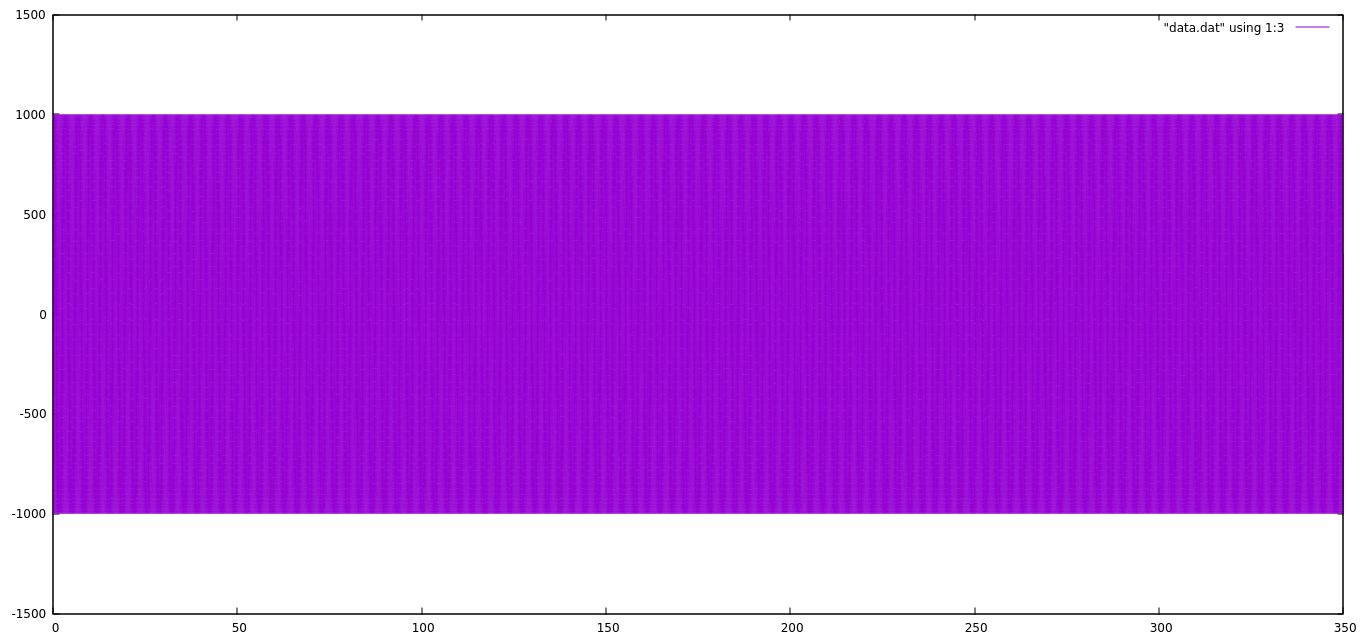
\includegraphics[scale=0.45]{period13.png}\\
\newpage
$[0,350]$ $x'(x)$ с точностью $10^{-11}$\\
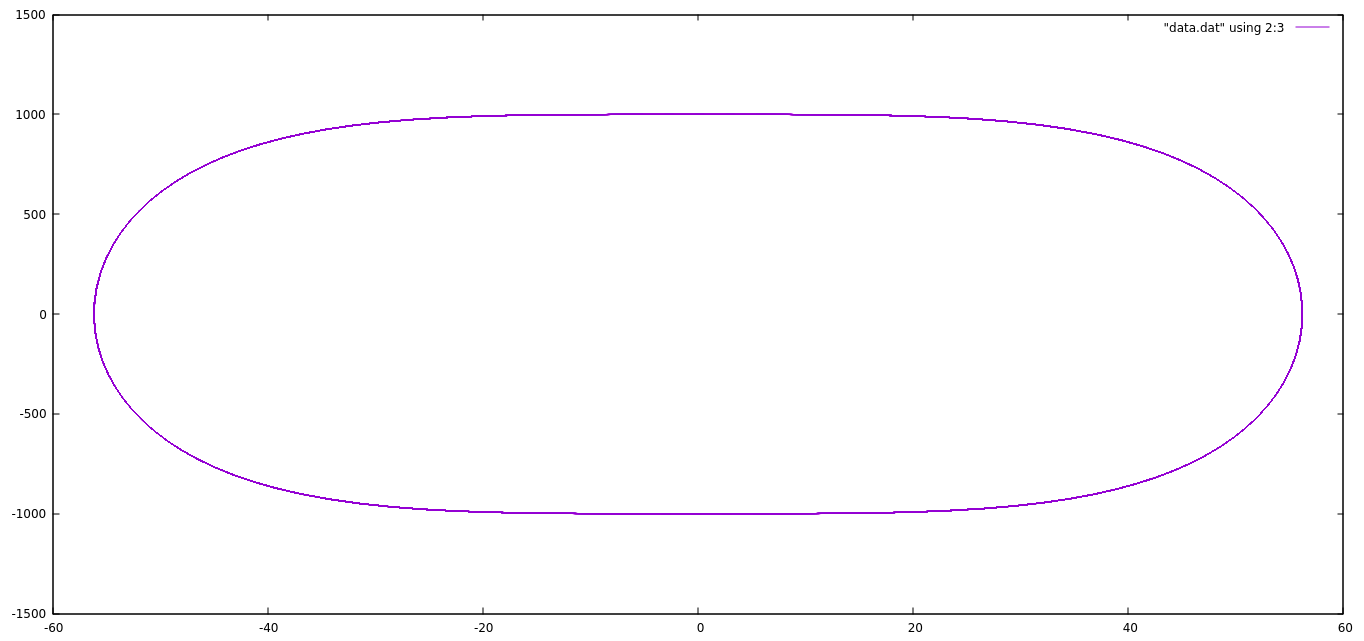
\includegraphics[scale=0.45]{period23.png}\\
\newpage
Рассмотрим теперь задачу для другого $\alpha$.
\begin{gather}
\begin{cases}
\notag x' = y \\
\notag y' = -(1 - 0.2x^2)x + cos(t) \\
\notag x(0) = 0 \\
\notag y(0) = 1
\end{cases}
\newpage
\end{gather}
\newpage
$[0,3.9]$ $x(t)$ с точностью $10^{-11}$\\
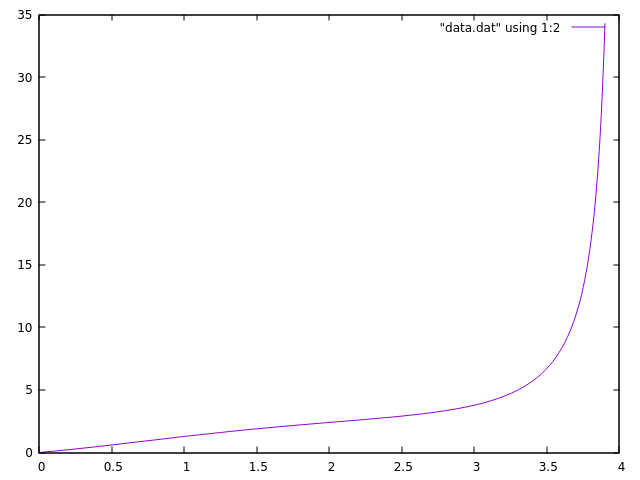
\includegraphics[scale=1]{neshod12.png}\\
\newpage
$[0,3.9]$ $x'(t)$ с точностью $10^{-11}$\\
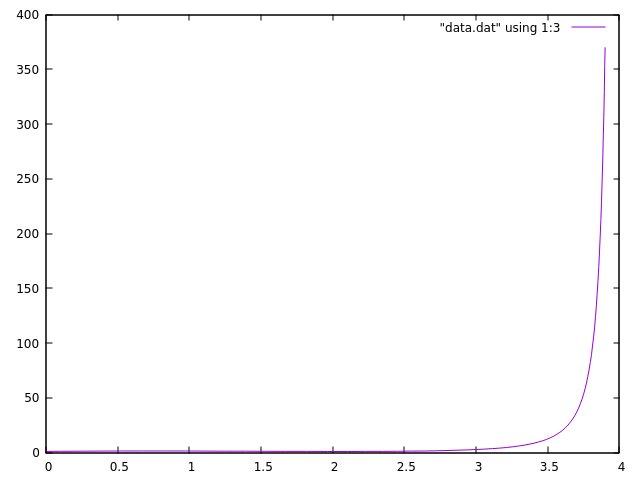
\includegraphics[scale=1]{neshod13.png}\\
\newpage
$[0,3.9]$ $x'(x)$ с точностью $10^{-11}$\\
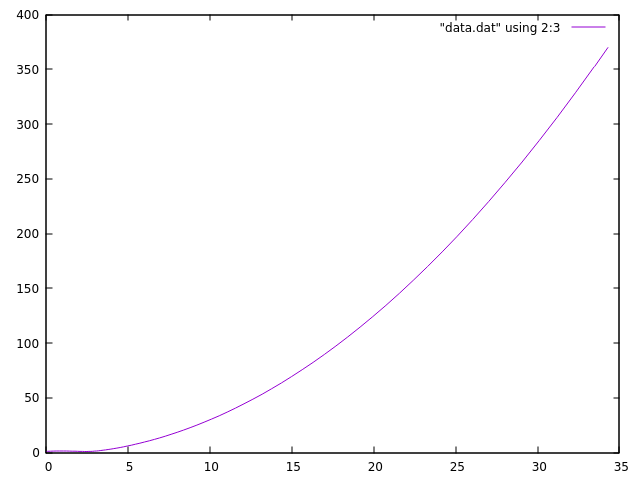
\includegraphics[scale=1]{neshod23.png}\\
\newpage Периода нет, Числа рунге $= 39.751736$ \\
 $x'(x)$ $[0, 3.99]$\\
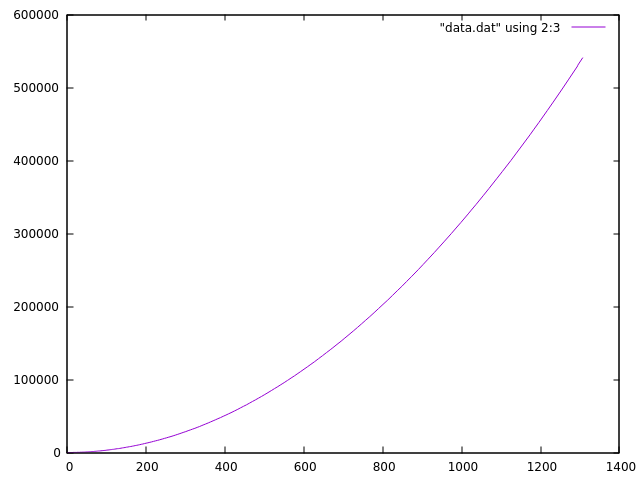
\includegraphics[scale=1]{neshod232.png}\\
\newpage

Нарисуем для нескольких начальных условий решения для $\alpha = 0.2$. Пусть $(x(0), y(0)) = {(0,2), (1,1), (2,0)}$ \\Числа Рунге соответственно: 40.815113, 40.815113, 50.875706\\
$[0,100]$ $x(t)$ с точностью $10^{-11}$\\
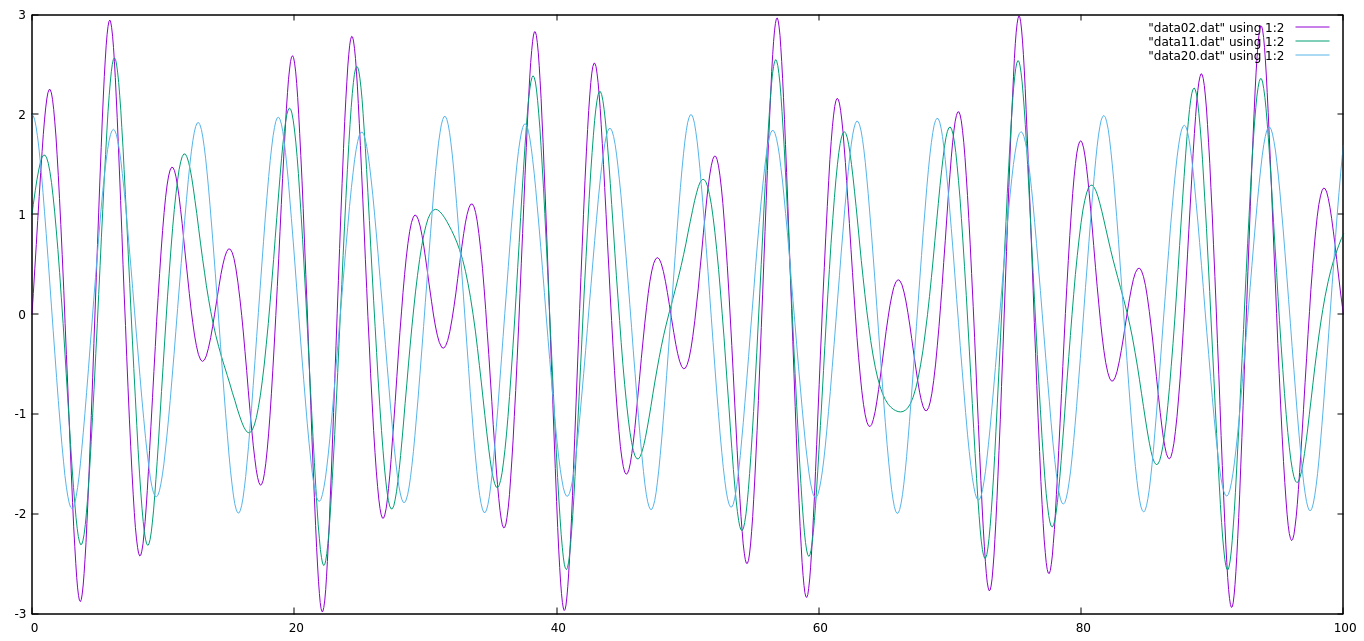
\includegraphics[scale=0.45]{0211201.png}\\
$[0,100]$ $x'(t)$ с точностью $10^{-11}$\\
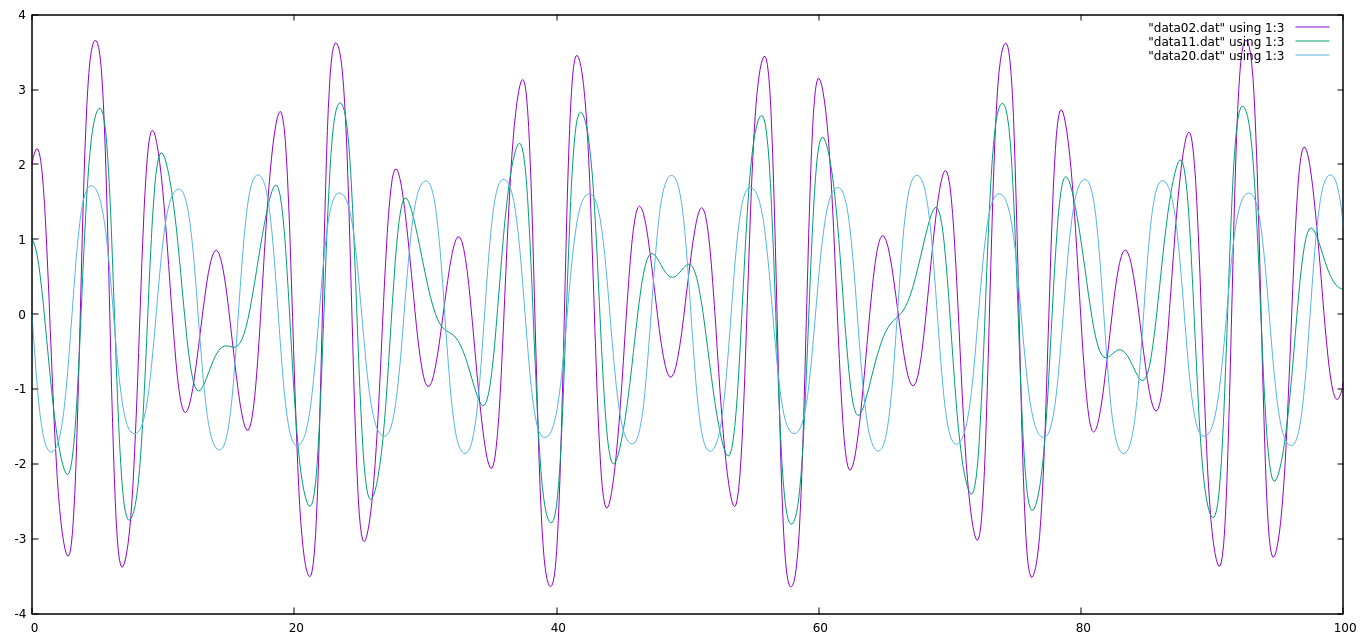
\includegraphics[scale=0.45]{0211202.png}\\
\newpage
$[0,100]$ $x'(x)$ с точностью $10^{-11}$\\
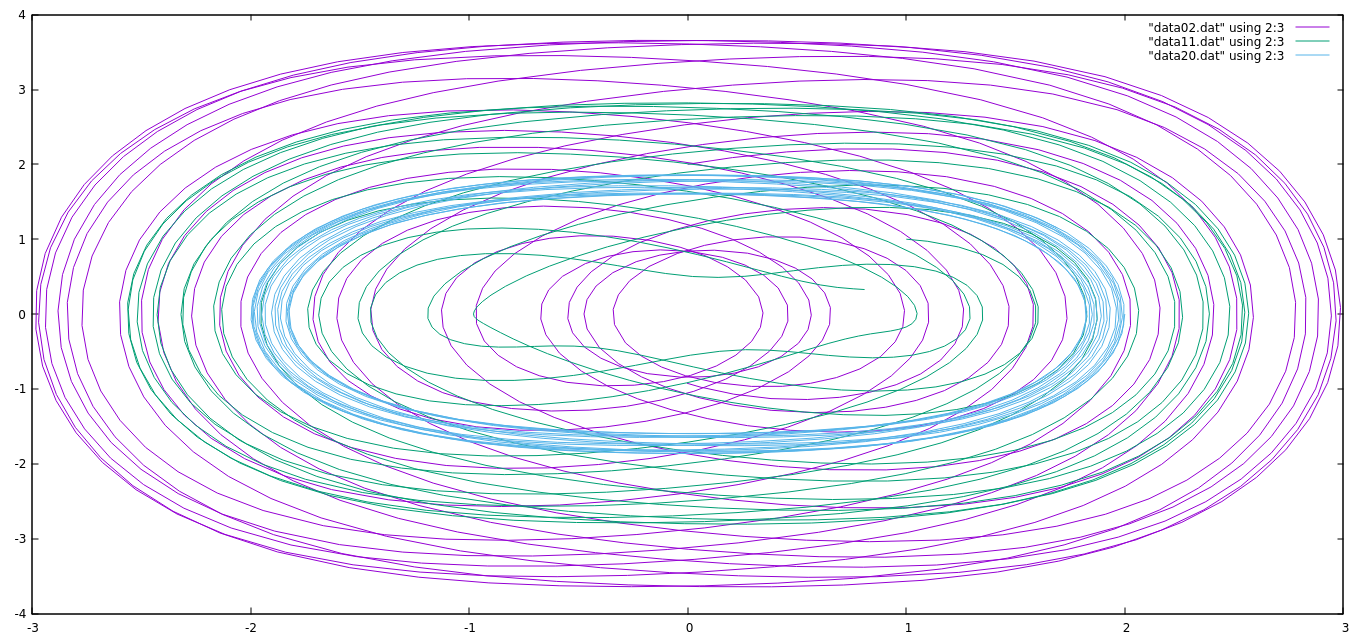
\includegraphics[scale=0.45]{0211203.png}\\
\newpage
Нарисуем для нескольких начальных условий решения для $\alpha = -0.2$. Пусть $(x(0), y(0)) = {(0,2), (1,1), (2,0)}$ \\Числа Рунге соответственно: 75.957517, 75.851, 75.935517\\
$[0,3]$ $x(t)$ с точностью $10^{-11}$\\
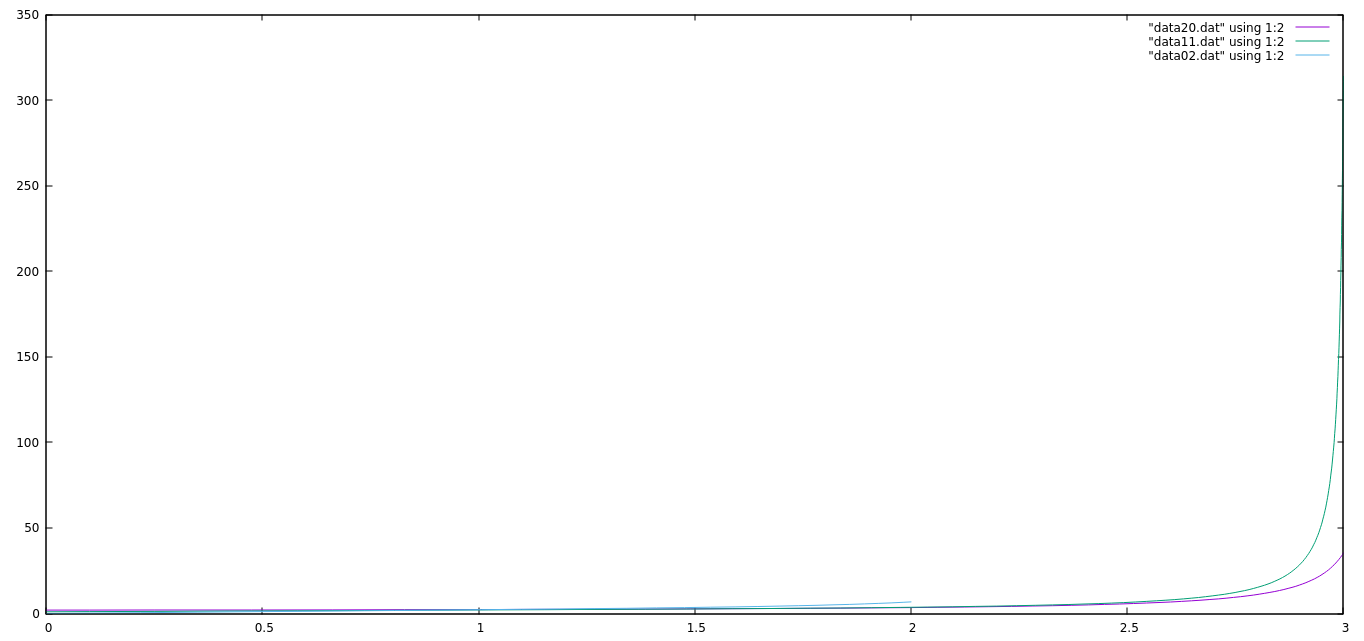
\includegraphics[scale=0.45]{rash31.png}\\
$[0,3]$ $x'(t)$ с точностью $10^{-11}$\\
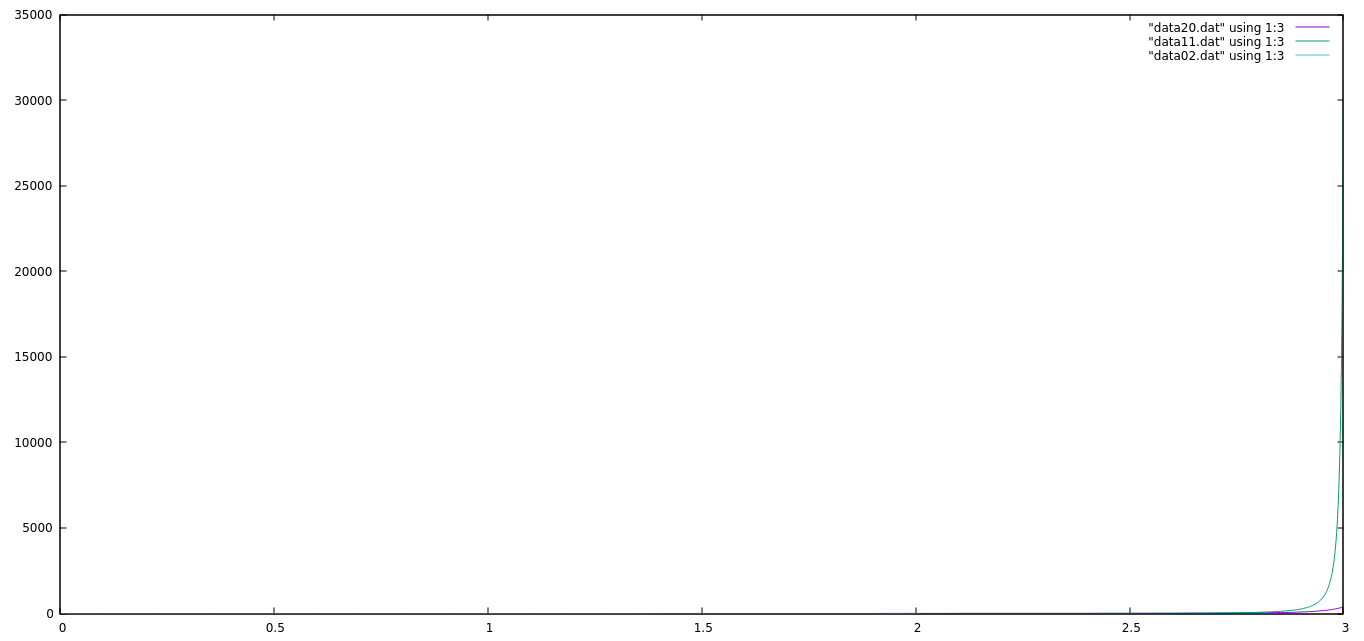
\includegraphics[scale=0.45]{rash32.png}\\
\newpage
$[0,2]$ $x'(x)$ с точностью $10^{-11}$\\
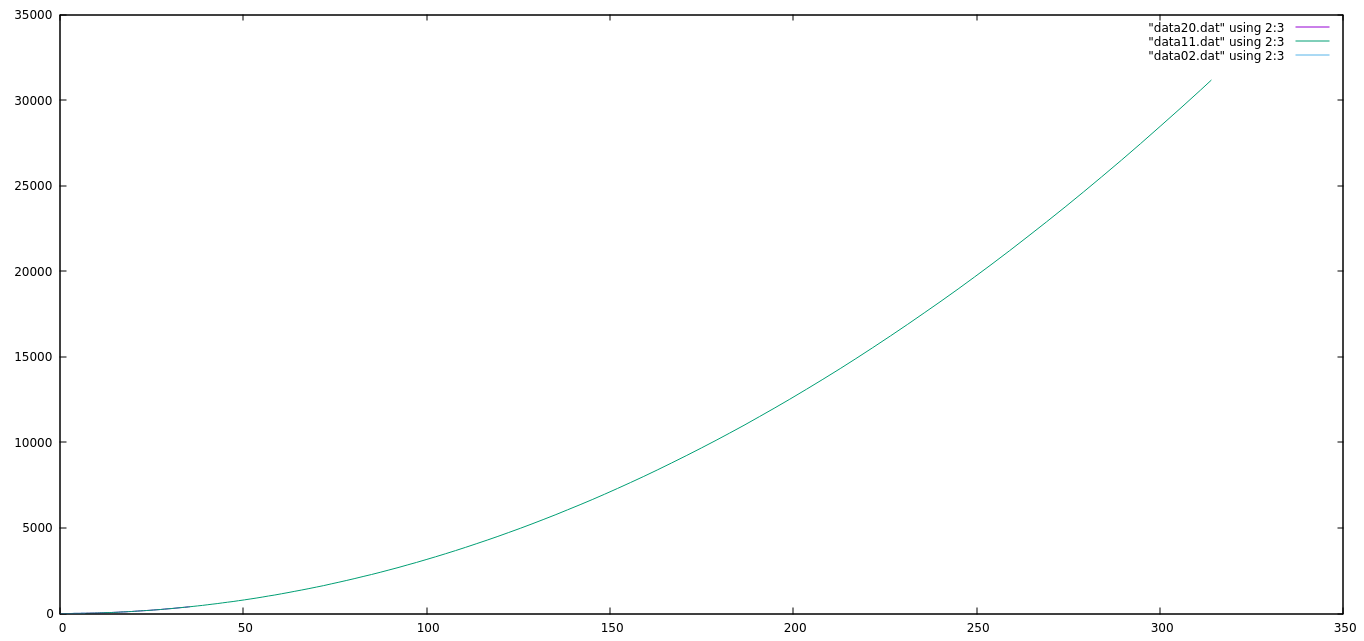
\includegraphics[scale=0.45]{rash33.png}\\
\newpage
\end{document}